\chapter{Grundlagen}
\label{Grundlagen}

\subsubsection{Framework}
Ralph E. Johnson in \cite{website:wiki-framework} definiert ein Framework wie folgt:
\begin{quote}
Ein Framework ist eine semi-vollständige Applikation. Es stellt für Applikationen eine wiederverwendbare, gemeinsame Struktur zur Verfügung. Die Entwickler bauen das Framework in ihre eigene Applikation ein, und erweitern es derart, dass es ihren spezifischen Anforderungen entspricht. Frameworks unterscheiden sich von Toolkits dahingehend, dass sie eine kohärente Struktur zur Verfügung stellen, anstatt einer einfachen Menge von Hilfsklassen.
\end{quote}
In dieser Arbeit dienen Frameworks oder auch Ordnungsrahmen zur Lösung spezieller Aufgaben und sind somit domänenspezifische Frameworks.
Das heißt, dass notwendige Funktionen und Strukturen zur Lösung von speziellen Aufgaben bereits vorhanden sind, die konkreten Lösungen müssen jedoch mit Hilfe des Frameworks erstellt werden.


\section{Datenbank}

\subsection{Begriffsdefinitionen}

\subsubsection{ACID}
Die bekanntesten Vertreter von relationalen Datenbanksystemen wie Oracle, MySQL und PostgreSQL arbeiten transaktional nach \Gls{acid}.
\Gls{acid} kann nach \cite{book:kudrass} S. 262 wie folgt definiert werden:
\begin{description}
\item[Atomarität] \hfill \\
Transaktionen sind atomar, wodurch ein Abbruch einer Transaktion deren enthaltenen Operationen rückgängig macht.
\item[Konsistenz] \hfill \\
Das Ende oder der Abbruch einer Transaktion geht immer mit Nachbedingung aller Intergritätsbedingungen einher.
\item[Isolation] \hfill \\
Transaktionen verschiedener Benutzer beeinflussen sich nicht gegenseitig.
\item[Dauerhaftigkeit] \hfill \\
Jede Änderung einer Transaktion ist nach Ende dieser auf die Festplatte geschrieben und nicht mehr im Puffer vorhanden.
\end{description}
Die Definition dieses anerkannten Begriffes ist für Kapitel \ref{nosql} notwendig.

\subsubsection{MVCC}
In grundlegenden relationalen Systemen werden Transaktionen verzögert oder sogar gesperrt, um Konsistenz und Isolation zu gewährleisten.
\Gls{mvcc} erhöht die Effizienz des  blockierenden Verhaltens.
Dabei werden von jedem Objekt mehrere Versionen verwaltet.
Neue Versionen entstehen durch Änderungen einer anderen.
Eine Transaktion verwendet die zu Transaktionsbeginn aktuelle Version.
Dadurch werden die allgemeinen Sperrverfahren (siehe \cite{book:kudrass} S. 266 ff.) verbessert, indem lesende Transaktionen sich nicht gegenseitig blockieren und schreibende- gegen lesende Transaktionen nicht mehr synchronisiert werden müssen. (vgl. \cite{book:kudrass} S. 270)

\subsubsection{BASE}
\Gls{base} ist ein optimistischer und sperrenfreier Ansatz mit fließender Konsistenz.
\cite{book:nosql-einfuehrung}

\subsubsection{CAP}
\Gls{cap}\\
TODO

%\subsubsection{Partition Tolerance}

%\subsubsection{Eventual-Consistency}

%\subsubsection{Consistent-Hashing}


%weitere Begriffsdefinitionen

\subsection{Indexstrukturen}

Indexstrukturen oder allgemein Zugriffsstrukturen dienen dem effizienten Zugriff auf Dateneinträge.
Ein Index ist nach \cite{book:kudrass} S. 284 wie folgt definiert:
\begin{quote}
Ein Index ist ein Verzeichnis von Dateneinträgen der Form (k, k*), das den effizienten Zugriff auf allen Einträgen mit einem Suchschlüsselwert k erlaubt. Dabei bezeichnet k den Wert eines Suchschlüssels (auch Zugriffsattribut) und k* den Verweis auf den Datensatz in der Datei, der k als Wert des Suchschlüssels enthält.
\end{quote}
Zugriffsstrukturen haben je nach Art und Umfang der Daten sowie entsprechend den Anforderungen an das \Gls{dbs} unterschiedliche Strukturen.
In der einfachsten Struktur unterscheidet man nach Indexen die direkt die Daten beinhalten, auf die Daten zeigen oder eine Menge von Adressen beinhalten. (siehe \cite{book:kudrass} S. 284)

Im folgenden werden spezielle Indexstrukturen vorgestellt, da dieses Wissen zur Bewertung von \Gls{dbs} herangezogen werden müssen.

\subsubsection{B-Baum}

\begin{quote}
Der B-Baum ist ein dynamisch balancierter Indexbaum, bei dem jeder Indexeintrag auf eine Seite der Hauptdatei zeigt.\footnote{\cite{book:kudrass} S. 288}
\end{quote}
Der Baum besitzt die Höhe h und die Ordnung m sowie die folgenden Eigenschaften:
\begin{quote}
1. Jeder Weg von der Wurzel zum Blatt hat die Länge h (balanciert)\\
2. Jeder Knoten enthält mindestens m Elemente (außer der Wurzel) und  höchstens 2m Elemente (mindestens halbvolle Belegung)\\
3. Jeder Knoten ist entweder eine Blattseite oder hat höchstens 2m + 1 Kinder (maximale Belegung)\footnote{ebenda}
\end{quote}
Diese Struktur garantiert eine Belegung von 50\%.
Weiterhin beschreibt h die Anzahl der Seitenzugriffe als relevantes Maß für die Zugriffskosten und Datensätze n bedingen den Zugriff in maximal logm(n) Seitenzugriffen. (vgl. \cite{book:kudrass} S. 288)

Eine Spezialisierung stellt der B+-Baum dar.
Hierbei befinden sich die Dateneinträge ausschließlich in den Blattknoten.
Die Blattknoten sind unidirektional verkettet.
%Ordnung ist hier (m -> Mindestbelegung für Indexseiten, m* -> Mindestbelegung der Blattseiten) m>m*

\subsubsection{LSM-Baum}
Log structured merge tree\\
TODO

\subsubsection{R-Baum}
R-Bäume sind balancierte Bäume und \glqq organisieren k-dimensionale Rechtecke mithilfe überlappender Blockregionen\grqq \ (\cite{book:kudrass} S. 523)
Diese Struktur wird folglich zur räumlichen Datenhaltung eingesetzt, da die Indexierung anhand räumlicher Informationen der Daten erfolgt.
Ein Verzeichnisknoten besteht aus einem Tupel (ref, mur).
ref steht für den Verweis auf den direkten Nachfahren und mur für das minimal umgebende Rechteck der Kindknoten.
Datenknoten enthalten dagegen nur mur als eigentliches Geoobjekt. (vgl. \cite{book:kudrass} S. 523 ff.)
% TODO: Bewertung!

\subsubsection{Geohash}
\label{geohash}
Bei Bedarf

\subsection{Mehrrechner-Datenbanksystem}

\begin{quote}
Bei einem Mehrrechner-Datenbanksystem (MDBS) werden die Datenbankverwaltungsfunktionen auf mehreren Prozessoren bzw. Rechnern ausgeführt.\footnote{\cite{book:kudrass} S. 394}
\end{quote}
Kudraß ergänzt dies durch folgende Unterscheidungen:
\begin{description}
\item[shared everything] \Gls{dbms} befindet sich auf eng gekoppelter Multiprozessor-Umgebung.
\item[shared nothing] Die Verarbeitung erfolgt durch mehrere Rechner mit jeweils einem \Gls{dbms}, dabei ist der Externspeicher unter den beteiligten Rechnern partitioniert.
\item[shared disk] Hierbei handelt es sich um mehrere lokal angeordnete, lose oder nah gekoppelte Rechner mit je einem \Gls{dbms} und einer gemeinsamen Speicherzuordnung. Lokal verteilte Systeme werden als parallele Datenbanksysteme bezeichnet.
\end{description}

\subsection{Verteiltes Datenbanksystem}

\begin{quote}
Verteilte Datenbanksysteme (VDBS) sind geografisch verteilte Shared-Nothing Systeme mit homogenen lokalen DBMS, die gemeinsam ein globales konzeptionelles DB-Schema unterstützen.
Förderierte Datenbanksysteme (FDBS) sind ebenfalls geografisch verteilte Sgated nothing systeme, wobei die beteiligten lokalen DBMS eine höhere Autonomie aufweisen, d.h. dass jeweils eine eigene lokale Datenbank mit lokalem DB-schema vorliegt.\footnote{\cite{book:kudrass} S. 398}
\end{quote}

\subsection{Replikationsverfahren}

\subsubsection{Synchron}\
Bei Bedarf

\subsubsection{Asynchron}\
Bei Bedarf

\subsubsection{Kaskadiert}\
Bei Bedarf

\newpage

\section{geografische Datenverarbeitung}

\subsection{Bezugssysteme}

\begin{quote}
Räumliche Bezugssysteme (spatial reference systems) erlauben die Interpretation der gespeicherten Koordinaten als Beschreibung von Lage- und Ausdehnungsinformationen in einem (realen) Datenraum. Ein räumliches Bezugssystem besteht aus einem Koordinatensystem (coordinate system), einem Geltungsbereich und Angaben, die es erlauben, Daten aus unterschiedlichen Koordinatensystemen auf ein globales System abzubilden.\footnote{\cite{book:kudrass} S. 506}
\end{quote}

Kudraß allgemeine Definition wird durch \cite{book:gi-theopluspraxis3} S. 141 ff. mit folgendem ergänzt:\\
Man unterscheidet Koordinatensysteme nach kartesisch, homogen, Kugeltransformation und Ellipsoidentransformation, wobei den kartesischen einer hoher Stellenwert zugegordnet wird.

Allen Bezugssystemen wird zur Identifikation ein weltweit eindeutiger Code zugeordnet.
Dieser ist ein von der European Petroleum Survey Group Geodesy vergebener so genannter EPSG Code.

Das auf einem Ellipsoiden basierende Bezugssystem World Geodetic System von 1984\footnote{EPSG:4326} wird von der Agricon GmbH verwendet.


\subsection{Datenformate}


\begin{quote}
Geoobjekte sind räumliche Elemente, die zusätzlich zu Sachinformationen geometrische und topologische Eigenschaften besitzen und zeitlichen Veränderungen unterliegen können. Kennzeichnend für Geoobjekte sind somit Geometrie, Topologie, Thematik und Dynamik.\footnote{\cite{book:gi-theopluspraxis3} S. 133}
\end{quote}
De Lange definiert räumliche Objekte bzw. Geoobjekte ausreichend.
Ein Geoobjekt enthält als Geometrie eine oder mehrere zwei- oder dreidimensionale Koordinaten, was die Lage, den Umfang und die Ausdehnung beschreibt.
Zur Topologie zählt de Lange Umgebungen, Nachbarschaften, Teilmengen und Überlagerungen.
Weiterhin werden Geoobjekte mit Sachinformationen gespeichert und je nach Anwendungsfall versioniert.[vgl. \cite{book:gi-theopluspraxis3} S. 133]


\subsubsection{einfache Geoobjekte}

Ein Punkt besteht aus einer zwei- oder dreidimensionalen Koordinate und beliebigen Sach-, Topologie- und Dynamikinformationen.
Mehrere Punkte bilden Linien.
Bildet eine Linie eine geschlossene Fläche, handelt es sich um ein Polygon.

\subsubsection{Vektorenmodell}

Es besteht die Möglichkeit eine Menge von Punkten als Vektoren aufzufassen und daraus topologische Objekte entstehen zu lassen.
Um damit geografisch zu modellieren, ist eine Diskretisierung d.h. eine Zuordnung der Vektoren notwendig. 

\subsubsection{Rastermodell}

Ein Raster löst einen rechteckigen Bereich mit in einem Koordinatensystem gleichmäßig angeordneten quadratischen Bildelementen bzw. Pixeln fester Größe auf.
Geodaten werden ergo mit einer indizierten Matrix abgebildet.
Ein dreidimensionales Raster heißt Voxel.
\begin{quote}
Ein Punkt wird näherungsweise durch ein einzelnes Pixel dargestellt. Ein Linienzug wird durch entsprechende Anordnungen zusammenhängender Pixel angenähert erfasst. Linienzüge können dann z.B. durch Folgen von Indexpaaren (Zeile, Spalte) der zugehörigen Pixel beschrieben werden. Eine Fläche ist ebenfalls durch zusammenhängende Pixel darstellbar. Somit sind keine weiteren Zusatzinformationen zur Modellierung von Flächen wie im Vektormodell notwendig [...].\footnote{\cite{book:gi-theopluspraxis3} S. 136}
\end{quote}


\subsubsection{Shapefile}\
Bei Bedarf

\subsection{Operationen}
% Grundlagenbuch geoinformatik zu rate ziehen

\subsubsection{Aggregation}
TODO

\subsubsection{Filterung}
TODO

\subsubsection{Geostatistik}
TODO

\subsubsection{Interpolation}
TODO

\subsubsection{Resampling}
Bei Bedarf


\subsection{GIS}
\label{grundlagen:gis}

Ein \Gls{gis} ist wie folgt definiert:
\begin{quote}
Ein System,  das  auf einen Datenbestand zurückgreift und Auswertungen dieser Daten zulässt,  so dass Informationen abgeleitet und wiedergegeben werden können,  kann  allgemein  als  ein  Informationssystem  bezeichnet  werden. [...]

Im Mittelpunkt  der  Geoinformatik  stehen  mit den  Geoinformationssystemen raumbezogene Informationssysteme, die im Gegensatz zu den übrigen Informationssystemen Geoobjekte  der realen Welt modellieren und diese in ein digitales Informationssystem abbilden [...]. Die Gegenstände eines Geoinformationssystems  besitzen  wie  auch  bei  allen  anderen  Informationssystemen  eine 
Thematik (und Dynamik). Das Besondere bei Geoinformationssystemen ist, dass Geoobjekte darüber hinaus Geometrie und Topologie als implizite und untrennbare Bestandteile aufweisen!  Die Verarbeitung derartiger raumbezogener Informationen erfordert spezielle Werkzeuge bzw. Funktionen, die von den übrigen Informationssystemen nicht bereitgestellt werden [...].\footnote{\cite{book:gi-theopluspraxis3} S. 337}
\end{quote}

%\subsection{GDAL}

\subsection{GeoTools}
\label{geotools}
GeoTools ist eine in Java geschriebene Open Source Bibliothek welche Standardkonforme Operationen zur Verarbeitung von geografischen Daten bereitstellt.
Die Implementation erfolgte nach Anforderungen des \Gls{ogc}, worauf beispielsweise Geometrien des \Gls{jts} unterstützt werden und die OGC Filter Encoding Spezifikation von Attributen und räumlichen Filtern verwendet wird.\footnote{vgl. \cite{website:geotools}}
\cite{website:geotools} listet die wichtigsten Funktionalitäten wie folgt auf:
\begin{quote}
\begin{itemize}
\item A clean data access API supporting feature access, transaction support and locking between threads
\begin{itemize}
\item Access GIS data in many file formats and spatial databases
\item Coordinate reference system and transformation support
\item Work with an extensive range of map projections
\item filter and analyze data in terms of spatial and non-spatial attributes
\end{itemize}
\item A stateless, low memory renderer, particularly useful in server-side environments.
\begin{itemize}
\item compose and display maps with complex styling
\item vendor extensions for fine control of text labels and color blending
\end{itemize}
\item Powerful schema asisted parsing technology using XML Schema to bind to GML content\\
The parsing / encoding technology is provided with bindings for many OGC standards including GML, Filter, KML, SLD, and SE.
\end{itemize}
\end{quote}
Unterstützte Formate sind nach der selben Quelle:
\begin{quote}
\begin{itemize}
\item raster formats and data access\\
arcsde, arcgrid, geotiff, grassraster, gtopo30, image (JPEG, TIFF, GIF, PNG), imageio-ext-gdal, imagemoasaic, imagepyramid, JP2K, matlab
\item Database “jdbc-ng” support\\
db2, h2, mysql, oracle, postgis, spatialite, sqlserver
\item Vector formats and data access\\
app-schema, arcsde, csv, dxf, edigeo, excel, geojson, org, property, shapefile, wfs
\item XML Bindings\\
Java data structures and bindings provided for the following: xsd-core (xml simple types), fes, filter, gml2, gml3, kml, ows, sld, wcs, wfs, wms, wps, vpf.\\
Additional Geometry, Filter and Style parser/encoders available for DOM and SAX applications.
\end{itemize}
\end{quote}


\subsection{PostGIS}
PostGIS ist eine geografische Erweiterung der Objekt-relationalen Datenbank PostgreSQL.
PostgreSQL wird dabei um geografische Datentypen, geografische Indizes und Funktionen erweitert.
Konkret wird der Simple Feature Access Standard verwendet und um den Datentyp raster und weitere Funktionen zur Datenverarbeitung erweitert. (siehe \cite{website:postgisdocu-opengis})
Somit kann mit SQL direkt mit geografischen Daten gearbeitet werden.
PostGIS steh unter der \Gls{gpl}v2.



\section{NoSQL}
\label{nosql}
\subsection{Definition}

NoSQL steht für eine Bewegung des letzten Jahrzehnts, in welcher die Abkehr von klassischen relationalen Systemen gefordert oder zumindest ein Umdenken bestehender Strukturen, Vorgehen und Grundsätze angestrebt wird.
Dies wird durch andere Abfragesprachen, nicht relationale Datenbanksysteme oder Neudefinitionen von Begriffen wie der Konsistenz zum Ausdruck gebracht.
Der Ursprung wird in der Literatur verschieden hergeleitet, jedoch wird immer zu den ersten Vertretern der NoSQL Bewegung Systeme mit einer anderen Abfragesprache und einfache Schlüssel-Hash Datenbanken gezählt.
Auf einer Messe zu aktuellen Trends im Datenbankbereich wurde der Begriff NoSQL zuerst öffentlich für Lösungen dieser Bewegung verwendet [vgl. \cite{website:originnosql}] und ist seitdem ein Sammelbegriff für eine hohe Anzahl an Systemen.

\subsubsection{NoSQL GIS}

In Bezug auf NoSQL kann \Gls{gis} wie in \ref{grundlagen:gis} definiert werden, jedoch muss das zugrunde liegende System nicht relational sein.
Im Rahmen dieser Arbeit ist mit \Gls{gis} ein System oder die Teilsysteme zur räumlichen Datenhaltung, Datenverarbeitung und Bereitstellung gemeint.

\subsection{Kategorisierung}
Edlich unterscheidet, wie andere Autoren, NoSQL Datenbanken nach vier Kategorien.
Jedoch kann eine eindeutige Zuteilung nicht für jedes System erfolgen, da Prinzipien verschiedener Kategorien auf eines zutreffen können.
Unter \url{http://nosql-database.org/} ist eine persönliche Übersicht der NoSQL Datenbanken von Herrn Edlich dargestellt.
Für dieses Kapitel diente wesentlich \cite{beamer:nosql} als Quelle.


\subsubsection{Key Value Datenbank}

Key Value Datenbanken speichern Daten in Tupeln aus Schlüssel und Wert.
Der Key ist eine Zeichenkette oder ein Hashwert und der Datentyp von Value ist beliebig im Rahmen der Datentypen der Datenbank.
Datenzugriff erfolgt über Key.
Es existiert keine einheitliche Abfragesprache.

Erste Datenbanken die zu NoSQL zugeordnet werden sind Key Value Datenbanken. Konkret DBM und BerkleyDB.
Aktuelle Vertreter sind Amazon Dynamo, Riak, Voldemort und Redis.

Diese Datenbanken eignen sich für heterogene Daten, horizontale Skalierung und Schemafreiheit, da diese einfach strukturierten Daten sich in keiner Relation zueinander befinden.

\subsubsection{Dokumentenbasierende Datenbank}

Hierbei werden strukturierte Daten, hier Dokumente, unter einem Hash abgelegt und sind über diesen abrufbar.
Diese Dokumente sind im großteil der dokumentenbasierten Datenbanken versioniert.
Häufige Formate sind \Gls{json}, \Gls{bson} und YAML.

Ziel ist hier schemafreie Daten zu speichern und den Zugriff zu skalieren.
Dabei können zumeist keine Joins verwendbar.

Bekannte Vertreter sind MongoDB, CouchDB und Terrastore.

\subsubsection{Spaltenorientierte Datenbank}

Im Gegensatz zu zeilenorientierten Datenbanken legen spalteniorientierte Datenbanken ihre Werte, hier Attribute einer Tabelle, spaltenweise ab.

Dies eignet sich für OLAP und Data Warehouse, da Spalteneinfügungen kostengünstig und Garbage Collection effektiv ist.
Dagegen besteht ein hoher Aufwand beim Lesen und Schreiben von zusammengehörigen Spaltendaten.

Googles Big Table erweitert diesen Ansatz und beschreibt es in dessen Paper wie folgt:
\begin{quote}
A  Bigtable  is  a  sparse,  distributed,  persistent  multi-dimensional sorted map. The map is indexed by a row key, column key, and a timestamp; each value in the map is an uninterpreted array of bytes.\footnote{\cite{paper:bigtable} S. 1}
\end{quote}
Die mehrdimensionalen Tabellen oder Maps sind vom Format:\\
$n*[Domain / Keyspace]\ x\ [item / Column\ Family]\ x\ [Key\ x]*n*[key+Value]$
%Dans zeug dazu anschauen

Googles Ansatz wurde OpenSource in HBase und Cassandra umgesetzt. Die konkrete Implementierung von Google wurde jedoch nicht veröffentlicht.
HBase verwendet folgendes Format: Pro Table Zugriff auf Zeilen per Rowkey, diese enthalten Column Familys oder Spalten welche wiederum eine Map namens Column Qualifier mit Tupeln aus der Version als Schlüssel und ein Byte-Array als Wert besitzt.[vgl. \cite{ba:dan} S. 13]

\subsubsection{Graphenbasierte Datenbank}

Der bekannteste Vertreter der graphenbasierten Datenbanken ist Neo4J.
Alle Daten und deren Beziehungen werden in Form von Graphen persistiert.
Ein Graph besteht dabei aus Knoten und gerichteten Kanten.
Knoten sind dabei strukturierte Objekte und Kanten Beziehungen zwischen den Objekten.
Diese strukturierten Objekte sind Key Value Tupel.
Kanten können typisiert sein.
Somit lassen sich direkt Beziehungen zwischen Daten definieren, was sich für semantic web, social network, Bioinformatik und Internetrouting eignet.

Diese Datenbanken sind nur optional mit einem Schema versehen und besitzen keine einheitliche Abfragesprache.
Auch sind im allgemeinen keine Joins vorgesehen.


\subsection{Hadoop}
\label{hadoop}
% http://blog.samibadawi.com/2012/03/hive-pig-scalding-scoobi-scrunch-and.html

Hadoop ist ein unter der Apache Lizenz 2.0 stehendes Java-Framework zur Datenhaltung und Verarbeitung von großen Datenmengen auf einem Verbund von mehrerern Computern.
Es basiert auf MapReduce und dem Dateisystem HDFS.

Das \Gls{hdfs} ist ein verteiltes Dateisystem, welches keine besonderen Anforderungen an die Hardware stellt und für die Verwendung von mehreren hundert bis tausend Computern\footnote{die in einem verteilten System teilnehmenden Computer heißen Knoten} ausgelegt ist.
Es besitzt eine hohe Fehlertoleranz und ist für den Einsatz auf kostengünstiger Hardware ausgelegt.
Hoher Datendurchsatz und die Verwendung großer Dateien\footnote{eine Datei kann mehrere Gigabyte bis mehrere Terrabyte groß sein und wird in Blöcke gleicher Länge aufgeteilt} sind wesentliche Merkmale.[vgl. \cite{paper:hadoop} S. 3]
Die Datei-Blöcke werden redundant auf die Knoten verteilt und sind mit Hilfe des Name-Node abrufbar.[vgl. \cite{ba:dan} S. 7]

Die verteilte Verarbeitung übernimmt MapReduce.
Entsprechend dem Namen entspringt der Name MapReduce aus der funktionalen Programmierung, in welcher die Funktionen \glqq map\grqq \ und \glqq reduce\grqq \ zum Einsatz kommen.
So werden hier die Daten mit einer map-Funktion verändert und mit reduce-Funktion aggregiert.
Ein Master weist die Daten und Funktionen den Slaves\footnote{In diesem Zusammenhang auch Worker genannt} zu.
Die Slaves führen die Funktionen mit den ihnen zugewiesenen Daten aus und speichern ihre Ergebnisse auf deren Festplatte ab.
MapReduce wurde von Google definiert.
In Abbildung \ref{fig:mapreduce} ist der beschriebe Ablauf dargestellt.
Auch hier werden keine besonderen Anforderungen an die Hardware gestellt.[vgl. \cite{paper:mapreduce} S. 3]

\begin{figure}[h]
\centering
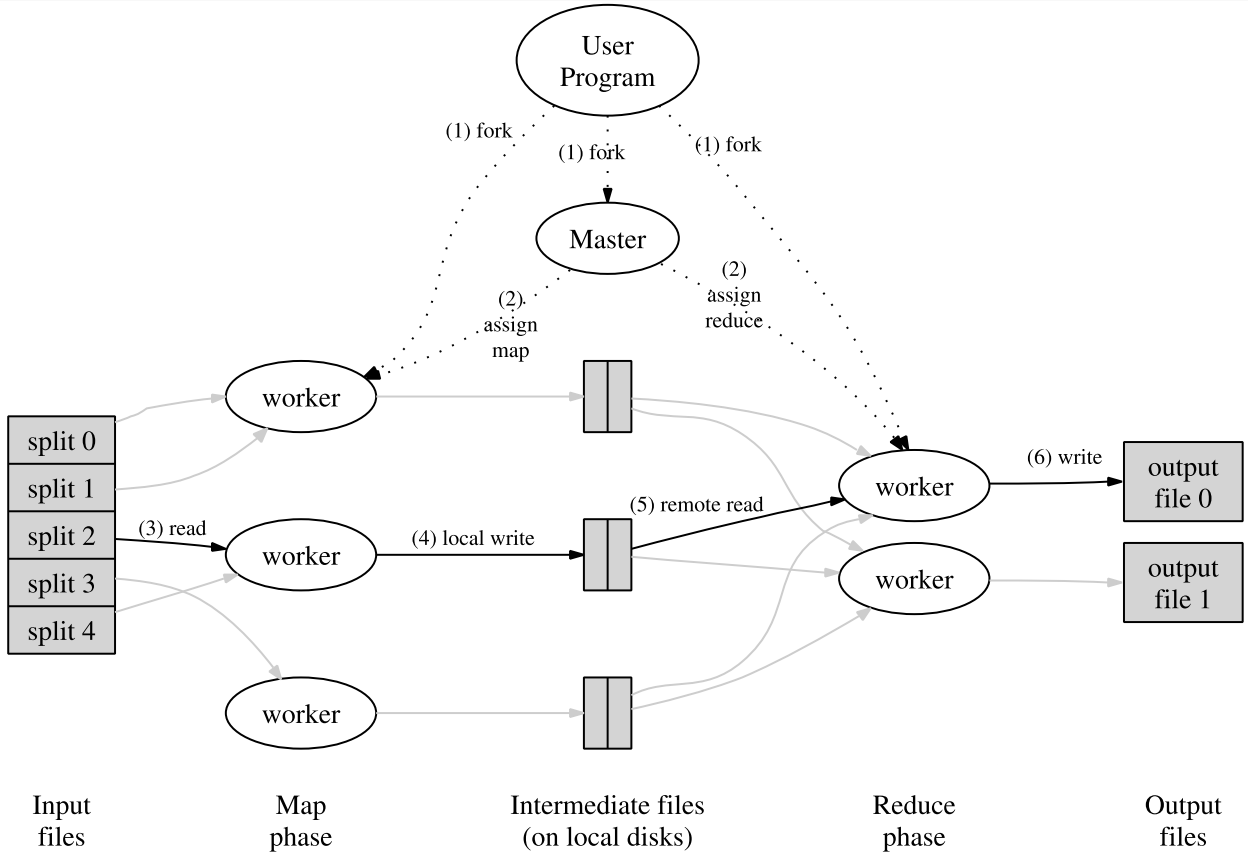
\includegraphics[width=\textwidth]{Abbildungen/mapreduce.png}
\caption[Übersicht der Ausführung von Googles MapReduce]{Übersicht der Ausführung von Googles MapReduce, Quelle: \cite{paper:mapreduce} S. 3}
\label{fig:mapreduce}
\end{figure}
%\begin{center}
%\centering
%\includegraphics[width=12cm]{Abbildungen/Testumgebung.png}%
%\captionof{figure}[Testumgebung]{Testumgebung}%
%\end{center}

Hadoop besitzt eine Master-Slave Architektur, wobei der Name-Node\footnote{damit ist der Master-Knoten gemeint, auch Jobtracker genannt} ankommende Anfragen bearbeitet und die Slave-Knoten organisiert.
Hadoop ist per API verwendbar und bietet sich somit zur Stapelverarbeitung an. %Todo: belegen
Es wird meist nur als Grundgerüst verwendet und mit Datenbanken wie HBase, MongoDB oder PostgreSQL sowie mit Frameworks für die Nutzung wie Hive, Pig, Spark oder Scalding erweitert.


\subsection{ZooKeeper}
\label{zookeeper}
Das Apache Projekt  ermöglicht verteilten Prozessen über ZNodes miteinander zu kommunizieren.
Es wird häufig gleichzeit mit Hadoop\footnote{siehe\ref{hadoop}} eingesetzt.
Ziel ist dabei ein hoher Durchsatz, geringe Latenzen, Hochverfügbarkeit und effektiver Zugriff durch die Prozesse.
Dabei verwaltet ZooKeeper eine geringe Datenmenge von einigen Kilobyte, da einzig Metainformationen von Interesse sind.\footnote{siehe \cite{website:zookeeper}} 



\subsection{Thrift}
\label{thrift}
\begin{quote}
The Apache Thrift software framework, for scalable cross-language services development, combines a software stack with a code generation engine to build services that work efficiently and seamlessly between C++, Java, Python, PHP, Ruby, Erlang, Perl, Haskell, C\#, Cocoa, JavaScript, Node.js, Smalltalk, OCaml and Delphi and other languages.\footnote{[\cite{website:thrift}]}
\end{quote}


\subsection{Accumulo}
\label{accumulo}
%https://en.wikipedia.org/wiki/Apache_Accumulo
Hierbei handelt es sich um ein Level-1-Apache Projekt, es ist eine Java Open-Source Implementation des BigTable Ansatzes von Google und wird seit 2008 entwickelt.
Es verwendet Hadoop\footnote{siehe\ref{hadoop}}, ZooKeeper\footnote{siehe \ref{zookeeper}} und Thift\footnote{siehe \ref{thrift}}.
Der BigTable Ansatz wird um Iteratoren, Zellenbezeichnungen, Constraints, Fragmentierungsmöglichkeiten einer dokumentbasierten Datenbank und die Unterstützung der gleichzeitigen Verwendung mehrerer HDFS namenodes erweitert.
Weitere Funktionen sind folgende:
\begin{itemize}
\item Verwendung mehrerer Master
\item Verwendung einer eigenen Zeitsynchronisation
\item Eingebaute temporäre Datenhaltung im Arbeitsspeicher
\item Bereitstellung von Testimplementierungen per API
\end {itemize}
Es existieren weiterhin verschiedene Erweiterungen zum Datenmanagement und Änderung des Ordnungsrahmens zur Verfügung.[\cite{website:accumulo_features}]

\subsection{GeoMesa}

GeoMesa ist eine freie\footnote{Apache License Version 2.0} geografische Datenbank der Firma LocationTech mit den Möglichkeiten der verteilten Verarbeitung und Versionierung von geografischen Daten.
Es erweitert Accumulo\footnote{siehe \ref{accumulo}},  unterstützt die GeoTools API und bietet ein Plugin für den Mapserver \Gls{geoserver} an.
Die Daten werden nach Geohash\footnote{siehe \ref{geohash}} verwaltet.[vgl. \cite{website:geomesaeclipse}]\\
GeoMesa wird in Verbindung mit stream processing\footnote{bspw. Spark oder Storm} und batch processing\footnote{bspw. Pig oder Cascading} verwendet.
Vorrangig werden Vektordaten von GeoMesa verarbeitet, durch eine optionale Erweiterung sind auch Rasterdaten verwendbar.
Dieses Framework ist in Scala geschrieben-

Datenimport wird ingest genannt, erfolgt über die Kommandazeile und unterstützt die Datenformate CSV, TSV und SHP.
CSV, TSV, Shapefile, GeoJSON, and GML können dagegen exportiert werden.


- Anderer Dateiimport mit GeoTools
- Verarbeitung nur über externe Tools (Spark, geotools)


\url{https://www.locationtech.org/proposals/geomesa} :\\
- outperforming postgis with geoserver


\url{http://de.slideshare.net/CCRinc/location-techdc-talk2-28465214}
- Verwendung fraktaler Kurven
- mit Spark und Scalding wesentlich schneller als PostGIS


\url{https://docs.google.com/presentation/d/1NO0ppk8MfDs8Q-QcUidZCSZK7YYwd9RjJoHV1V4Yq_w/edit?pli=1#slide=id.p} :\\
- 

%storm vs spark: http://xinhstechblog.blogspot.de/2014/06/storm-vs-spark-streaming-side-by-side.html https://stackoverflow.com/questions/24119897/apache-spark-vs-apache-storm http://www.zdatainc.com/2014/09/apache-storm-apache-spark/


%https://github.com/locationtech/geomesa

%\subsection{Neo4J}

\subsection{Postgres-XL}
Postgres-XL ist ein frei verfügbares Clustersystem für PostgreSQL unter der Mozilla Public License.
XL steht dabei für eXtensible Lattice, erweiterbarer Verbund.
Damit soll es ermöglicht werden, mit PostgreSQL verteilt Schreiboperationen zu skalieren sowie parallele Datenverarbeitung auf mehreren physischen und virtuellen Systemen gleichzeitig zu betreiben.
Dafür wird zur verteilten Datenhaltung \Gls{acid} mit \Gls{mvcc} und zur parallelen Verarbeitung ein \Gls{mpp} Mechanismus eingesetzt. (siehe \cite{website:postgresxl-about})
Die Postgres-XL Umgebung nutzt mehrere PostgreSQL Instanzen oder Partitionen und bietet eine Schnittstelle für alle Instanzen an.\\
Abbildung \ref{fig:postgresxl} verbildlicht den Aufbau.
Laut Abbildung wird als erstes ein Load-Balancer angesprochen.
Dies wird in der Dokumentation nicht belegt.
Die anderen Elemente sind nach \cite{website:postgresxl-about} wie folgt beschrieben:
\begin{description}
\item[Global Transaction Manager] Dient als Verwaltungselement der Transaktionen und realisiert \Gls{mvcc} über das System. Laut Dokumentation existiert für jedes PostgreSQL Element ein GTM, um \Gls{mvcc}  mit je einem globalen Kontext realisieren zu können.
\item[Coordinator] \glqq The Coordinator manages the user sessions and interacts with GTM and the data nodes. The Coordinator parses and plans queries, and sends down a serialized global plan to each of the components involved in a statement.\grqq\ (\cite{website:postgresxl-overview})
\item[Data Node] Diese Elemente enthalten PostgreSQL. Diese müssen sich nicht eine Datenbank replizieren, sondern können auch eine Datenbank über partitioning teilen. Anfragen können von verschiedenen Coordinators gleichzeitig in unterschiedlichen Sitzungen erfolgen. Auf Grund der Kapselung besitzt jeder Data Node seinen eigenen Kontext zur Transaktion.
\end{description}
\begin{figure}[h]
\centering
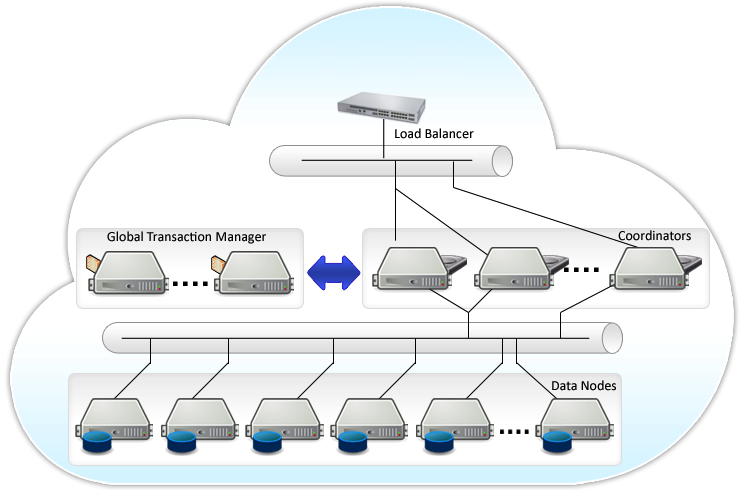
\includegraphics[width=.7\textwidth]{Abbildungen/postgresxl-structure.jpg}
\caption[Aufbau Postgres-XL]{Aufbau Postgres-XL, Quelle: \url{http://www.postgres-xl.org/wp-content/uploads/2014/04/xl_cluster_architecture1.jpg}}
\label{fig:postgresxl}
\end{figure}
Das System wird analog einer PostgreSQL Instanz angesprochen.
Ebenso ist PostGIS verwendbar.

\subsection{Rasdaman}

Rasdaman ist ein Array-Datenbanksystem speziell zum speichern und verarbeiten von Rasterdaten.
Es erweitert eine relationale Datenbank und wird mit  multi-dimensionalität der Daten, einer eigenen SQL ähnlichen Abfragesprache, Parallelisierung und Skalierbarkeit in beliebigen Maßstab sowie OGC konformen Diensten beworben.
Es ist als Client bzw. API unter der \Gls{lgpl} 3 und als Server unter der \Gls{gpl} 3 für Linux, MacOS und Solaris verfügbar.
Als OGC konforme Dienste werden WMS 1.3, WCS 2.0, WCS-T 1.4, WCPS 1.0 und WPS 1.0 bereitgestellt.
Die API kann in Java, C++ und über die eigene Abfragesprache rasql verwendet werden.[vgl. \cite{website:rasdamanogeo}]
Der beschriebene Aufbau ist unter Abbildung \ref{fig:rasdaman} dargestellt.

Es besteht die Möglichkeit, Rasdaman zu einer bestehenden PostgreSQL zu installieren und direkten Datenaustausch zwischen den beiden Systemen zu ermöglichen.
Weiterhin kann Rasdaman in Verbindung mit GDAL verwendet werden.
Momentan existiert eine Community und eine Enterprise Variante. Dabei verfügt die Enterprise Variante über mehr Features wie beispielsweise Datenkomprimierung, Serververwaltung per Webbrowser, Laufzeitoptimierungen und verschiedene Datenbankschnittstellen.
Von der verwendeten Datenbank wird BLOB als Datenbankinterner Datentyp verwendet.[vgl. \cite{website:rasdamanowiki}]
\begin{figure}[h]
\centering
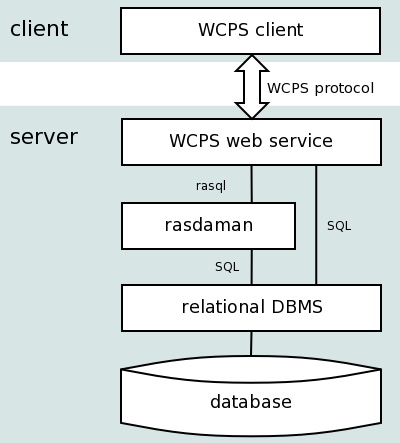
\includegraphics[width=.4\textwidth]{Abbildungen/rasdaman-aufbau.png}
\caption[Aufbau Rasdaman]{Aufbau Rasdaman, Quelle: \url{http://www.rasdaman.org/raw-attachment/wiki/Technology/wcps-stack.png}}
\label{fig:rasdaman}
\end{figure}

\subsection{Spacebase}

Spacebase ist eine in Java programmierte geografische Datenbank mit Betonung auf Echtzeit und geringe Latenzen des Unternehmens Parallel Universe.
Die Datenbank wird ausschließlich im Arbeitsspeicher gehalten und ausgeführt.
Außerdem ist sie für die verteilte Nutzung auf mehreren Computern konzipiert.
Räumliche Daten werden in 2D oder 3D mit einem dazugehörigen begrenzenden Rechteck im R-Baum gespeichert.
SpaceBase ist für eine sehr große Anzahl an Abrufen und Veränderungen der Daten in Echtzeit geeignet.
Für die räumliche Verarbeitung stehen Bereichsabfragen, Überschneidungsabfragen und allgemeine Join Abfragen zur Verfügung.
Diese beschränken sich aber auf das begrenzende Rechteck, da die eigentliche Geometrie nur über eine Referenz im Datenobjekt abrufbar ist.
Ergänzend besteht die Möglichkeit eigene Abfragen zu formulieren und dabei die referenzierte Geometrie zu verwenden.
Es wird jedoch darauf hingewiesen, dass complexe Operationen auf diese Geometrie die Laufzeit der Berechnungen wesentlich erhöht.
Zum Erreichen der geringen Latenzen werden räumliche Berechnungen parallelisiert und auf die Instanzen verteilt.
Es stehen APIs für Java, C++, Erlang, Python, Ruby und Node.js zur Verfügung.[vgl. \cite{website:spacebase}]


\subsection{ESRI GIS Tools for Hadoop}
Das Unternehmen ESRI stellt eine Umgebung zum verteilten Verarbeiten geografischer Daten auf einem Hadoop Cluster bereit.
Diese Umgebung nennt sich GIS Tools for Hadoop und besteht aus vier Teilen:
\begin{description}
\item[Esri Geometry API for Java] Java API für Entwickler, um mit Hadoop geografische Datenverarbeitung durchzuführen. JSON, WKT und Shapefile sind Importformate. Die Datentypen werden als einfache Geometrien bezeichnet und setzen sich laut Quellcode aus Punkt, Punktsammlung, Linie, Polygon und PolyLine zusammen. Geografische Funktionen sind \glqq union, difference, intersect, clip, cut, and buffer\grqq \ sowie \glqq equals, within, contains, crosses, and touches\grqq . (vgl. \cite{website:esrigishadoopapi})
\item[Spatial Framework for Hadoop] Erweiternte Bibliothek für Hadoop, um mit HQL geografisch zu arbeiten.
\item[Geoprocessing Tools for Hadoop] Hadoop Anbindung an ArcGIS.
\item[GIS Tools for Hadoop] Projekt zum testen der Hadoop Umgebung mit ArcGIS.
\end{description}
ArcGIS ist ein proprietäres GIS, die beschriebene Umgebung steht dagegen unter Apache Lizenz Version 2.0 zur Verfügung.(vgl. \cite{website:esri-hadoop2})

\section{Tests}

Die zu analysierenden Systeme sind mit Hilfe von Tests zu untersuchen und zu vergleichen.
Diese Tests müssen einerseits vergleichend sein, ergo bei unterschiedlichen Systemen die gleichen Merkmale testen und wiederholbar sein, andererseits die relevanten Merkmale testen.

Es handelt es sich somit um systematische Tests:
\begin {quote}
Ein systematischer Test ist ein Test, bei dem\\
die Randbedingungen definiert oder präzise erfasst sind,\\
die Eingaben systematisch ausgewählt wurden,\\
die Ergebnisse dokumentiert und nach Kriterien beurteilt werden, die vor dem Test festgelegt wurden.\footnote{\cite{book:softwareengineering} S. 446}
\end{quote}

Nachfolgend werden die Randbedingungen definiert und in Kapitel \ref{Anforderungen} die Ein- und Ausgaben dargestellt.


\subsection{Funktionstests}
\label{grundlagen-funktionstests}
Um die Systeme auf Softwarequalität, beschrieben auf Seite \pageref{softwarequalität}, zu testen, sind Funktionstests notwendig.
\cite{book:softwareengineering} verweist auf Funktionstests auf Seite 455 wie folgt:
\begin{quote}
Werden die Testfälle auf Basis der in der Spezifikation geforderten Eigenschaften des Prüflings ausgewählt (z.B. Funktionalität, Antwortzeit), dann spricht man von einem Block-Box-Test oder auch von einem Funktionstest (19.5).
\end{quote}
Dazu wird auf Seite 471 der Umfang des Funktionstestes wie folgt umrissen:
\begin{quote}
Ein umfassender Black-Box-Test sollte\\
alle Funktionen des Programms aktivieren (Funktionsüberdeckung),\\
alle möglichen Eingaben bearbeiten (Eingabeüberdeckung),\\
alle möglichen Ausgabeformen erzeugen (Ausgabeüberdeckung),\\
die Leistungsgrenzen ausloten,\\
die spezifizierten Mengengrenzen ausschöpfen,\\
alle definierten Fehlersituationen herbeiführen.
\end{quote}
Im Rahmen dieser Arbeit soll dieser Umfang wie folgt begrenzt werden:
\begin{description}
\item[Funktionsüberdeckung] Zur Einschätzung der Eignung eines Systems für den Anwendungsfall sind ausgewählte Funktionen zu testen, Im allgemeinen besitzen die ausgewählten Systeme Funktionen die in diesem Rahmen nicht genutzt werden sollen, jedoch auch Funktionen die von Hand ergänzt werden müssen. Die notwendige Menge an Funktionen soll einzig getestet und somit abgedeckt werden.
\item[Eingabeüberdeckung] Auch hierbei stehen verschiedene von den Systemen bereitgestellte Schnittstellen und Austauschformate zur Verfügung, aber es sollen nur die relevanten untersucht werden.
\item[Ausgabeüberdeckung] siehe Eingabeüberdeckung
\item[Leistungsgrenzen] Dafür werden eigene Tests definiert und verwendet.\footnote{siehe \ref{Leistungstests}}
\item[Mengengrenzen] Die zu untersuchenden Systeme eignen sich zum Speichern großer Datenmengen die mehrere Terrabyte bis Petabyte umfassen. Da die vorhandenen Datenmengen diese Größe unterschreitet, müssen die Mengengrenzen nicht wesentlich getestet werden.
\item[Fehlersituationen] Es besteht nicht das Ziel die Fehleranfälligkeit als einzelnes Merkmal zu untersuchen, weshalb dafür keine Testfälle erstellt oder durchgeführt werden. Einzig die Korrektheit der Berechnungen wird überprüft, indem die Ergebnisse des aktuellen ist-Standes zum Vergleich herangezogen werden. 
\end{description}

\subsection{Leistungstests}
\label{Leistungstests}

- Lasttests zur Persistierung von Eingangsdaten
- Lasttests zur Bereitstellung von verarbeiteten und eingabedaten (an UMN[plugin, WMS, Bilder oder über pgsql] oder allgemein)
- Überwachung der Systemauslastung ist notwendig

Ein Kriterium der Untersuchung in dieser Arbeit ist die Leistung.
Nach Kesselman in \cite{book:Leistungsanalyse} S. 20 ist Leistung die gewichtete Summation von Leistungsindizes, wobei ein Leistungsindex die Quantifizierung einer Eigenschaft eines Systems ist.
Wesentliche Leistungsindizes sind Laufzeiten von einfachen oder komplexen Operationen.
Es wird hier nur die spezielle Leistung gemessen, da ausgewählte Eigenschaften betrachtet werden und somit nicht die Leistung für einen allgemeinen Anwendungsfall.

Der in diesem Zusammenhang in der Literatur verwendete Begriff Benchmark ist hier jedoch ungeeignet, da die Software und nicht die Hardware untersucht werden soll:
\begin {quote}
Benchmarking ist eine Methode der Analyse des Leistungsverhaltens von Rechensystemen anhand von Referenzprogrammen oder Sätzen von Referenzprogrammen (Benchmarks). Dabei wird das Leistungsverhalten verschiedener Rechensysteme in Relation gesetzt, um so Vergleichskriterien  für Rechensysteme zu erhalten.\footnote{\cite{book:Leistungsanalyse} S. 24}
\end{quote}
Eine hier betrachtete Leistungs- und Laufzeitmessung ist dabei wie folgt definiert:
\begin {quote}
Unter Leistungsmessung versteht man die Beobachtung des Ablaufverhaltens eines Programms bei der Ausführung auf einem realen System. Das Ziel das dabei verfolgt wird, ist die Gewinnung von Erkenntnissen, die zur Optimierung eines Programms genutzt werden können.\footnote{\cite{book:Leistungsanalyse} S. 28}
\end{quote}
Die aus der Leistungsmessung gewonnenen Erkenntnisse dienen hierbei als Qualitätsmerkmale und werden nach definierten Metriken gewichtet.

%Leistungsmessungen des \Gls{tpc} werden zum Zwecke der vergleichenden Leistungsfeststellung von Software 
Es existieren vordefinierte Leistungstests, dabei sind jene des \Gls{tpc} sowie die Benchmarks 001, 007, HyperModel und Justitia zu nennen.
Diese sind jedoch nicht für den zu untersuchenden Anwendungsfall geeignet, da sie die allgemeine Leistungsfähigkeit und Effektivität messen und somit nicht die gesuchten Werte der \Gls{gis} ermitteln.